\newpage

\section{Acoustic modeling}

\subsection{Discrete HMMs in continuous space}

In ASR terminology, an HMM is \textit{discrete} if the output space is partitioned into discrete, non-overlapping regions. The most common way to find such regions is to use $k$-means clustering. Then, the HMM states can emit discrete indices identifying one particular region.

A simple example of this is the regular partitioning of the F1-F2 formant space.

\subsection{Source coding}

\begin{itemize}
    \item Scalar quantization:
        \begin{itemize}
            \item for a scalar observation $x$, compute a quantization $y = Q(x)$
            \item can be simple, such as rounding (e.g. $1.3 \rightarrow 1.0$ or $1.3948 \rightarrow 1.40$)
        \end{itemize}
    \item Vector quantization:
        \begin{itemize}
            \item divide large set of vectors into groups using e.g. $k$-means clustering
            \item identify vectors by their group index
            \item lossy data compression
        \end{itemize}
\end{itemize}

\subsection{Continuous HMMs}

In ASR terminology, an HMM is \textit{continuous} when the output space is continuous and so are the emission probabilities $b_i$. Often, Gaussians $b_i = \mathcal{N}(\mu_i, \Sigma_i)$ are used ($\mu_i$ is a $k$-dimensional vector, $\Sigma_i$ is a $k \times k$ covariance matrix).

It is also possible to use a mixture of Gaussians:

\[
    b_i = \sum\limits_{j=1}^M c_{ij} \mathcal{N}(\mu_{ij}, \Sigma_{ij}) \mbox{\hspace{15pt} (or rather: \hspace{5pt}} b_i = \sum\limits_{j=1}^M c_{ij} \mathcal{N}(\mu_{j}, \Sigma_{j}) \mbox{\hspace{5pt} ?)}
\]

where $c_{ij}$ are the mixture weights.

If time is not an issue, we can use a continuous model. Otherwise, we will have to save computation time by altering our model.

\subsubsection{Conversion to semi-continuous model}

We ``pull out'' each Gaussian and collect them in a codebook. There will be a maximum of $M \cdot N$ Gaussians, where $N$ is the number of states and $M$ is the number of mixtures (different gaussians).

\subsubsection{Conversion to shared semi-continuous model}

We extend the mixture weights to include Gaussians that were initially assigned to other states. This means that many mixture weights which previously were $0$ are now greater than $0$. This results in even more parameters.

\vspace{15pt}

\textbf{Problem:} If we create one codebook for each emission probability, we end up with \textit{a lot of} parameters. We may not have enough data to train our model.

\vspace{5pt}

\textbf{Solution:} Parameter tying. The most flexible way of parameter tying is to use an arbitrary number of Gaussian codebooks and an arbitrary number of mixture weight sets.

\subsubsection{Conversion to tied semi-continuous model}

Reduce the size of the codebook to a smaller size $L < M \cdot N$. Share Gaussians that belong to similar units (\textit{tie units}). This ``ties'' the codebook elements (and states) together. The number of models to train is now manageable.


\subsection{Discrete vs. Continuous HMMs}
\begin{itemize}
\item Feature space is small and discrete? - Use discrete HMMs
\item Feature space is small and continuous? - Try discretization (vector quantization)
\item Feature space is large? - (semi)continuous probably works best
\item Data set is small? - discrete (fast, compact and little training but low precision) vs. continuous (complementary properties)
\end{itemize}

\subsection{Parameter tying}

There are two main approaches to parameter tying:
\begin{itemize}
    \item \textbf{Knowledge driven:} Have an expert sit down and decide which parameters to tie.
    \item \textbf{Data driven:}
        \begin{itemize}
            \item let $n$ be the number of training vectors for a codebook, set the codebook size to $n \cdot f$ where $f$ is an empirically found factor
            \item run $k$-means with different values for $k$, choose the $k$ with the best result
            \item start with one codebook, train, once we have enough data, split
            \item start with huge codebook, remove Gaussians with too few training counts, retrain
            \item merge and split
        \end{itemize}
\end{itemize}

The following parameters can be tied:
\begin{itemize}
    \item sets of Gaussians
    \item within a mixture: have different Gaussians use the same covariance matrix
    \item transitions: different HMM states share the same transition probabilities
\end{itemize}

\subsection{Lexicon}

\textbf{Problem:} How do we connect our HMMs to words?

\vspace{5pt}

\textbf{Solution:} With a pronunciation dictionary.

\vspace{10pt}

In the simplest architecture, a word is represented as a sequence of phonemes and each HMM state represents one phoneme. In the lexicon, each word is bound to a phoneme sequence.

\subsubsection{Pronunciation variants}

One word can be pronounced differently due to:
\begin{itemize}
    \item coarticulation effects
    \item dialects (e.g. \textit{thing} vs. \textit{thang})
    \item various correct pronunciations (e.g. a = AE or a = EY)
    \item correct pronunciation differs from most commonly used ones (e.g. \textit{February} vs. \textit{Febyury})
\end{itemize}
To solve this problem, we add variants to the pronunciation dictionary. When building an HMM for a word, we build multiple, alternative state sequences.
\\
How do we find Pronounciation variants?
\begin{itemize}
\item Linguist \emph{Problem:} Often linguistic units dont correspond to acoustic units
\item ASR Expert \emph{Problem:} Often most successful approach but also very expensive 
\item Problems for both approaches: Inconsistencies
\item Automatic Dictionary Learning: 
\begin{itemize}
\item train a phone based recognizer
\item Run recognition on word based segmented data
\item Single out the top-N most frequent phoneme sequences per word
\item Add these sequences as pronounciation to the dictionary
\item Problems: accuracy of phone recognizer, requires lots of segmented data
\end{itemize}

\end{itemize}


\subsection{Context dependent acoustic modeling}

Consider the pronunciation of \textit{train} and \textit{tell}. Common lexicon entries will be \textit{T-R-EY-N} and \textit{T-EH-L}, but the actual pronunciation often sounds more like \textit{CH-R-EY-N} and \textit{T-HH-EH-L}. The phoneme \textit{T} sounds different depending on the phoneme following it.

At first, one might try to alter the lexicon entries, i.e. \textit{CH-R-UW} instead of \textit{T-R-UW}, but the \textit{CH} in \textit{true} sounds different from the one in \textit{church}.

So, we introduce new acoustic units, such that lexicon entries might look like \textit{T(R)-R-EY-N} and \textit{T(vowel)-EH-L}. This means that we use context-dependent models of the phoneme \textit{T}.

\subsubsection{Crossword context modeling}

It is not a good idea to assume that the left context of a word is silence. Because of this, we extend context modeling across word boundaries while building a sentence HMM.

\textit{Go to AM1 26/30 for more on this subject.}

\subsubsection{Position dependent modeling}

The same phoneme (with the same context) is pronounced differently depending on its position in the word. As an example, consider the \textit{D}-phoneme in \textit{Idaho} and \textit{my dad}. To solve this problem, we use position dependent modeling, where \textit{wb} indicates a word boundary. In \textit{Idaho}, this will become \textit{D(AY, AE)}, whereas in \textit{my dad}, it will become \textit{D(wb)(AY, AE)}.

\subsubsection{Parameter tying}

With so many different states, even with lots of training data, the HMM cannot be trained enough. As a solution, we use parameter tying to combine multiple contexts into the same context class:

\begin{itemize}
    \item Knowledge based:
        \begin{itemize}
            \item let a linguist define classes $C_i$ of phonemes (e.g. vowels, consonants, fricatives, etc.)
            \item then, define generalized triphones for a monophone $M$: $M(C_l, C_r)$
        \end{itemize}
    \item Data driven:
        \begin{itemize}
            \item use some algorithm with an optimization criterion to decide which contexts should be tied
        \end{itemize}
    \item Backoff procedure:
        \begin{itemize}
            \item if we have enough training data for triphones, use triphones $P_m(P_l, P_r)$
            \item otherwise, if we have enough training data for left or right context biphones ($P_m(P_l)$ or $P_m(P_r)$), use them
            \item otherwise, as a fallback, use an indepent model $P_m$
        \end{itemize}
\end{itemize}

\subsection{Clustering}

There are two different approaches to clustering:
\begin{itemize}
    \item \textbf{bottom-up clustering} (agglomerative): start with one class for each phone, then combine ``similar enough'' classes until satisified
    \item \textbf{top-down clustering} (divisive): start with one class for all phones, divide a class if it seems like a ``good idea'', continue until satisfied
\end{itemize}

Both approaches result in a \textit{clustering tree}.

\vspace{10pt}
\textbf{Problem:} How do we know whether it's a good idea to separate a class? 

\vspace{5pt}

\textbf{Solution:} Use a \textit{distance measure}.
\vspace{10pt}

\subsubsection{Continuous parametric models}
\begin{itemize}
    \item $d(f, g) = \int \min(f(x), g(x))$
    \item Kullback-Leibler divergence: $d_{KL}(f, g) = \int f(x) \ln \frac{f(x)}{g(x)}$
    \item entropy distance: $d(f, g) = H(f + g) - \frac{1}{2} H(f) - \frac{1}{2} H(g)$
    \item Notice: We want to minimize d because it signals information-loss due to lost parameters
\end{itemize}

\subsubsection{Discrete models}
Semi-continuous and discrete HMMs are represented by \textit{discrete} distributions.
\begin{itemize}
    \item $H(f) = \sum\limits_i f[i] \log_2(\frac{1}{f[i]})$
    \item $d(f, g) = H(f + g) - \frac{1}{2} H(f) - \frac{1}{2} H(g)$
    \item obviously: $f = g \Rightarrow H(f) = H(g) = H(f + g) \Rightarrow d(f, g) = 0$
\end{itemize}

As an example, consider $f = \left\{\frac{1}{2}, \frac{1}{2} \right\}$, $g = \left\{\frac{3}{4}, \frac{1}{4} \right\}$. Then, $f + g = \left\{\frac{5}{8}, \frac{3}{8} \right\}$. It follows that $H(f) = 1$, $H(g) \approx 0.81$, $H(f + g) \approx 0.95$ and finally $d(f, g) \approx 0.05$.

\vspace{10pt}

\textbf{Weighted discrete entropy distance}

\vspace{5pt}

Consider three models $M_1, M_f, M_{f^+}$, where $M_1$ is a model trained with many samples, $M_f$ is a model trained with few samples and $M_{f^+}$ is a model that is trained with few samples, but more than $M_f$ was trained with. Combining $M_1$ with $M_f$ should have a smaller impact on the distance compared to combining $M_1$ with $M_{f^+}$. Thus, we weigh the model entropy by the number of training samples:

\[
    d(f, g) = (n_f + n_g) H(f + g) - n_f H(f) - n_g H(g)
\]

\subsubsection{Kai-Fu Lee}
\begin{enumerate}
    \item train semicontinuous models for all three states of each triphone, e.g. triphone \textit{A(AE,K)-b} \textit{A(AE,K)-m} \textit{A(AE,K)-e}.
    \item initialize a context class for every triphone (a context class is defined by three distributions, e.g. \textit{$T_{17}$-b}, \textit{$T_{17}$-m}, \textit{$T_{17}$-e})
    \item compute all distances between different context classes of same phone:
        \[
            d(C_i, C_j) = E(C_i\mbox{\textit{-b}}, C_j\mbox{\textit{-b}}) + E(C_i\mbox{\textit{-m}}, C_j\mbox{\textit{-m}}) + E(C_i\mbox{\textit{-e}}, C_j\mbox{\textit{-e}})
        \]
    \item replace the two classes with the smallest class by their combination
    \item try to improve distance by moving any element from any class into any other class
\end{enumerate}

\vspace{10pt}
\textbf{Note:} This algorithm is completely data driven. Step 5 is expensive but important.
\vspace{10pt}

Kai-Fu Lee's algorithm produces \textit{generalized triphones}. For example, \textit{A(H,U)} and \textit{A(B,P)} might be combined into \textit{A37}, and \textit{A(L,N)} and \textit{A(M,M)} might be combined into \textit{A38}.

\subsubsection{Decision trees}

After clustering, we might end up with two classes:
\[
    C_1 = \left\{P_1(P_2, P_3), P_1(P_4, P_5) \right\} \mbox{\hspace{20pt}} C_2 = \left\{P_1(P_6, P_7), P_1(P_8, P_9) \right\}
\]
\textbf{Problem:} If we want to recognize the word sequence $P_3, P_1, P_7$, do we use $C_1$ or $C_2$ to model $P_1(P_3, P_7)$?

\vspace{5pt}

\textbf{Solution:} Build a decision tree.

\vspace{10pt}

\begin{enumerate}
    \item initialize one cluster containing all contexts
    \item for all clusters and questions: compute distance of subclusters
    \item perform the split that gets the largest separation
    \item continue until satisfied
\end{enumerate}

See figure~\ref{fig:growDecisionTree} for an example.

\begin{figure}[ht]
\centering
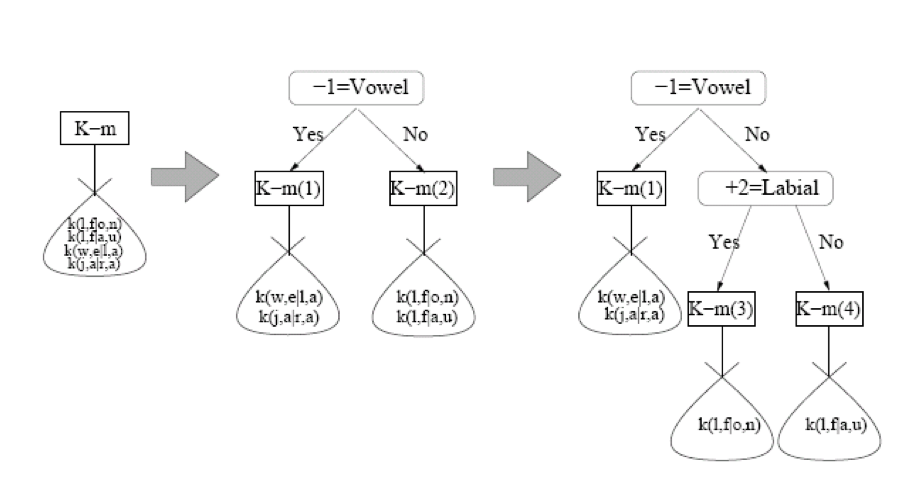
\includegraphics[width=10cm]{images/decision.png}
\caption{Decisiontree}
\label{fig:growDecisionTree}
\end{figure}

\textbf{Note:} It doesn't matter which questions we ask, as long as our question set allows for a variable enough separation.

\newpage

\section{Language modeling}

Remember the fundamental problem of speech recognition:

\[
    \argmax_W P(X \bigm| W) \cdot P(W)
\]

The purpose of the language model is to compute the probability $P(W)$ of a word sequence $W = (w_1, \ldots, w_n)$. \\
A LM should \dots
\begin{itemize}
\item improve speech recognizer by adding another independent information source.
\item disambiguate homophones, e.g.: \textit{``I OWE YOU TOO''} vs \textit{``EYE O U TWO''}.
\item reduce search space since not all word sequences are possible.
\item Analysis to \emph{understand} utterance, disambiguate homonyms (bank: money vs river).
\end{itemize}

\subsection{Deterministic vs. Stochastic Language Models}
 
In formal language theory (see Chomsky hierarchy) $P(W)$ is either 0 or 1. One way to model a deterministic language is with grammars. This deterministic approach is unsuitable for ASR because spoken language can not be completely covered by grammar and is often ungrammatical, anyway. Thus, stochastic LMs, e.g. \emph{N-grams}, are employed.

\subsection{N-grams}

The difficulty of recognizing a word sequence is correlated to the \textit{branching degree}. For example, the branching degree of \textit{``I apologize for being late, I'm very ---!''} is smaller than the one of \textit{``Hello, my name is ---.''}.

The choice of the next word depends on the entire history. Since there are too many histories to test them all, we have to find equivalence classes $\mathcal{C}$ so that:
\[
    P(w \bigm| \mbox{history}) = P(w \bigm| \mathcal{C}(\mbox{history}))
\]

We can use different equivalence classes using information about:
\begin{itemize}
\item grammatical content
\item Part-of-Speech (POS) of previous word(s)
\item semantic meaning of previous word(s)
\item context similarity
\item some kind of automatic clustering
\end{itemize}

A simple, yet common choice for the equivalence classes are $N$-grams:
\[
    P'(w_k \bigm| w_1, \ldots, w_{k-1}) = P(w_k \bigm| w_{k - (n - 1)}, \ldots, w_{k-1})
\]

Usually, $P(w \bigm| \mbox{history})$ is estimated by counting relevant occurances:
\[
    P(w \bigm| \mbox{history}) = \frac{Count(\mbox{history} \cdot w)}{Count(\mbox{history})}
\]

$N$-grams are helpful because in HMM-recognizers the language model is responsible for the computation of the transition probabilites between acoustic models on a word level.
They can be computed on the fly and may depend on previous words.

\subsubsection{Bigrams vs. Trigrams}

While Bigrams can be easily worked into an HMM-recognizer (you only need to take $w_t$ into consideration for the probability of $w_{t+1}$), Trigrams often require a larger history, especially if a word can have many predecessors.

Possible solutions are to use a \emph{time asynchronous search} or use so-called \emph{poor man's trigrams} (e.g. consider only the predecessor's best predecessor).

Additionally the test data coverage of Trigrams is smaller than with Bigrams and the estimation of  $P(w_k \bigm| w_{k - 2}, w_{k-1})$ is more difficult than $P(w_k \bigm|  w_{k-1})$.

\subsection{Perplexity}

To compare to different language models, we need an independent measure. Since the performance of a recognizer not only depends on the Language model, but also the acoustic model and the combination mechanism of the acoustic model with the language model, we use \emph{perplexity}.

A language model is ``good'' if it has a low \textit{perplexity}. The perplexity $PP$ of a language model $P$ on the test set $W = (w_1, \ldots, w_n)$ is:
\[
    PP = P(w_1, \ldots, w_n)^{-1/n} ( = 2^{H(W)})
\]

\subsection{Smoothing}

The key problem of $n$-grams is the \textit{data sparseness} problem: many n-grams will not occur in the training data, and many others will only occur very few times, resulting in inaccurate calculations. For example, in a several million word collection of English text, 50\% of trigrams occur only once, and 80\% of trigrams occur less than 5 times. As a start, we assign all strings a non-zero probability, in an effort to prevent ASR errors.

The idea of smoothing is to ``free probability mass'' from well-trained events and ``redistribute'' it to unseen events. This is somewhat similar to the idea of taxation.

\subsubsection{``Add-one'' smoothing}

Add 1 to all bigrams:

\begin{eqnarray*}
    P_{one}(w_i \bigm| w_{i - 1}) &=& \frac{C(w_{i-1}w_i)+1}{C(w_{i-1}) + n_v} \\
                                  &=& (1 - \lambda(w_{i-1})) \frac{C(w_{i-1}w_i)}{C(w_{i-1})} + \lambda(w_{i-1}) \frac{1}{n_v}
\end{eqnarray*}

where $\lambda(w_{i-1}) = n_v \bigm/ (n_v + C(w_{i-1}))$ and $n_v = \left|\left\{w : C(w) > 0 \right\} \cup \left\{\mbox{UNK} \right\}\right|$. This means that we're mixing the estimated distribution with the uniform distribution. However, when $n_v$ gets large, the estimation approximates the uniform distribution.

\subsubsection{Backoff smoothing}

Whenever possible, use higher-order models. Otherwise, for example with unseen events, backoff to lower-order models.
\begin{equation*}
    P_{bo}(w_i \bigm| w_{i-1}) = \begin{cases}
        \tilde{P}(w_i \bigm| w_{i-1}) & \mbox{if } C(w_{i-1}w_i) > 0 \\
        \lambda(w_{i-1}) \cdot P_{bo}(w_i) & \mbox{otherwise}
                                 \end{cases}
\end{equation*}

\vspace{20pt}
\textbf{Absolute discounting}
\vspace{10pt}

Subtract a fixed $D$ from each $n$-gram count:
\begin{equation*}
    P_{abs}(w_i \bigm| w_{i-1}) = \begin{cases}
        \frac{\max(C(w_{i-1}w_i)-D, 0)}{C(w_{i-1})} & \mbox{if } C(w_{i-1}w_i) > 0 \\
        \lambda(w_{i-1}) \cdot P_{abs}(w_i) & \mbox{otherwise}
                                 \end{cases}
\end{equation*}

\vspace{10pt}

\textit{\textbf{Note:} This formula is probably incorrect. I think what we're trying to do is something like this:
    \begin{equation*}
        P_{abs}(w_i \bigm| w_{i-1}) = \begin{cases}
            \frac{C(w_{i-1}w_i) - D}{C(w_{i-1})} & \mbox{if } C(w_{i-1}w_i) > D \\
            \lambda(w_{i-1}) \cdot P_{abs}(w_i) & \mbox{otherwise}
        \end{cases}
    \end{equation*}
    Or possibly even a weighted approach.
}

\vspace{20pt}
\textbf{Good-Turing estimation}
\vspace{10pt}

The idea is to reallocate the probability mass of $n$-grams that occur $r+1$ times in the training data to the $n$-grams that occur $r$ times. In particular, reallocate the probability mass of $n$-grams that were seen once to the $n$-grams that were never seen.

For each count $r$, we compute an adjusted count $r^\ast$:
\[
    r^\ast = (r+1)\frac{n_{r+1}}{n_r}
\]
where $n_r$ is the number of $n$-grams seen exactly $r$ times. Then, we compute the discount $d_r$:
\[
    d_r = \frac{r^\ast}{r}
\]

\vspace{20pt}
\textbf{Katz smoothing}
\vspace{10pt}

Use $k$ as a threshold to apply discounting. Use Good-Turing for discounting.
\begin{equation*}
    P_{katz}(w_i \bigm| w_{i-1}) = \begin{cases}
                                       \frac{C(w_{i-1}w_i)}{C(w_{i-1})} & \mbox{if } r > k \\
                                       d_r \cdot \frac{C(w_{i-1}w_i)}{C(w_{i-1})} & \mbox{if } k \geq r > 0 \\
                                       \alpha(w_{i-1}) \cdot P_{katz}(w_{i}) & \mbox{if } r = 0
                                   \end{cases}
\end{equation*}

\vspace{20pt}
\textbf{Kneser-Ney smoothing}
\vspace{10pt}

As an example, let's suppose that ``San Francisco'' is common, but ``Francisco'' occurs only after ``San''. Then ``Francisco'' will get a high unigram probability and so absolute discounting will give a high probability to ``Francisco'' appearing after novel bigram histories (for example, ``Los Francisco''). Since ``Francisco'' only ever occurs after ``San'', it is better to give it a low unigram probability. All in all, we use absolute discounting with a special backoff function. Define:
\begin{eqnarray*}
    \#(\bullet \; w_i) &=& \left|\left\{w_{i-1} : C(w_{i-1}w_i) > 0 \right\}\right| \\
    \#(\bullet \; \bullet) &=& \sum\limits_{w_i} \#(\bullet \; w_i)
\end{eqnarray*}

Then, define:
\[
    P_{KN}(w_i) = \frac{\#(\bullet \; w_i)}{\#(\bullet \; \bullet)}
\]

\subsubsection{Linear interpolation}

Define:
\[
    P_I(w_i \bigm| w_{i-2}w_{i-1}) = \lambda \cdot \tilde{P}(w+i \bigm| w_{i-2}w_{i-1}) + (1 - \lambda) \cdot P_I(w_{i} \bigm| w_{i-1})
\]

Key difference: in the case of non-zero counts, interpolated models still use information from lower-order models while backoff models do not.

(Deleted Interpolation Smoothing)

\subsection{$n$-gram classes}

Another way to handle data sparsity is to group words into classes of similar semantic or grammatical behavior. For simplicity, let's assume that one word $w_i$ can be assigned to only one class $c_i$. Then:
\[
    P(w_i \bigm| c_{i-(n-1)}, \ldots, c_{i-1}) = P(w_i \bigm| c_i) \cdot P(c_i | c_{i-(n-1)}, \ldots, c_{i-1})
\]

$n$-gram classes have not improved recognition accuracy significantly.

\subsection{Different kinds of language models}

\subsubsection{Cache language models}
\begin{itemize}
    \item \textbf{Idea:} Use a static and a dynamic component.
    \item \textbf{Static component:} $P_S(w_k \bigm| w_{k-(n-1)}, \ldots, w_{k-1})$, i.e. the usual trained language model.
    \item \textbf{Dynamic component:} Complete $n$-gram language model constructed from the text dictated so far, e.g.:
        \[
            P_C(w_k \bigm| w_{k-(n-1)}, \ldots, w_{k-1}) = \frac{1}{2} \cdot f(w_k) + \frac{1}{4} \cdot f(w_k | w_{k-1}) + \frac{1}{4} \cdot f(w_k | w_{k-2} w_{k-1})
        \]
    \item \textbf{Total language model:} $P_T = \lambda_C \cdot P_C + (1 - \lambda_C) \cdot P_S$
    \item \textbf{Variation:} Compute $P_C$ on last $l$ words of cache, vary $\lambda_C$ with cache size.
\end{itemize}

\subsubsection{Trigger language models}
\begin{itemize}
    \item \textbf{Observation:} Often, when a content-carrying word occurs in a text, it is likely to occur again some time later.
    \item \textbf{Idea:} Use a standard interpolated $n$-gram model, but constantly update the unigram probabilities $P(w_k)$ for some words $w_k$.
    \item \textbf{Trigger:} For each word $w$ define a trigger list $L(w)$ of words that are likely to occur some time later, e.g. $L(\mbox{money}) = \left\{\mbox{bank}, \, \mbox{savings}, \, \mbox{dollars}, \, \ldots \right\}$
    \item Then, for each word $v \in L(w)$, increase $P(v)$ by some value.
\end{itemize}

\subsubsection{Multilevel language models}
\begin{itemize}
    \item \textbf{Idea:} Use language models $LM_W$ for word sequences, $LM_P$ for phrases and $LM_S$ for sentences trained as regular $n$-gram grammars over their corresponding segments of speech.
    \item \textbf{Combination:} Let the total language model $LM_T$ be a combination of the three models:
        \[
        LM_T = \lambda \cdot LM_W + \lambda \cdot LM_P + \lambda \cdot LM_S
        \]
\end{itemize}

\subsubsection{Interleaved language models}
Sentences can often be split into two separate word sequences, one containing \textit{content words} and the other containing \textit{non-content words}:
\[
\begin{array}{|r|ccccccc|}
    \hline
    \mbox{\textbf{sentence:}} & \mbox{The} & \mbox{president} & \mbox{of the} & \mbox{software company said} & \mbox{that they will} & \mbox{introduce} & \mbox{...} \\
    \hline
    \mbox{\textbf{non-content:}} & \mbox{The} & & \mbox{of the} & & \mbox{that they will} & & \mbox{...} \\
    \mbox{\textbf{content:}} & & \mbox{president} & & \mbox{software company said} & & \mbox{introduce} & \mbox{...} \\
    \hline
\end{array}
\]

Based on this, we define:
\[
    P(w \bigm| \mbox{history}) = \begin{cases}
        P_C(w \bigm| C_1(\mbox{history})) & \mbox{if $w$ is a content word} \\
        P_{NC}(w \bigm| C_2(\mbox{history})) & \mbox{if $w$ is a non-content word}
    \end{cases}
\]

\subsubsection{Morpheme-based language models}
In heavily inflicted or agglutinating languages, the word stem is succeeded or preceded by gender-, tempus-, numerus- and case-identifying elements. The probabilities of full words cannot be estimated robustly. However, a robust estimation can be given for the word stem. So, we don't compute the language model on sequences of words but on sequences of morphemes:
\[
    P(w_1, \ldots) = \tilde{P}(w_{11}, w_{12}, \ldots, w_{1n_1}, \ldots)
\]

\subsubsection{Context-free grammar language models}
Context-free grammars can be used instead of $n$-grams. The rules of the grammar can be written by an expert without the need for lots of training data. CFGs are powerful enough to represent large parts of natural languages and constrained enough to allow for efficient search space reduction. Furthermore, semantic analysis of speech is possible with CFG-derived finite state automata ($\to$ figure~\ref{fig:contextFreeGrammarLM}).

\begin{figure}[htb]
\centering
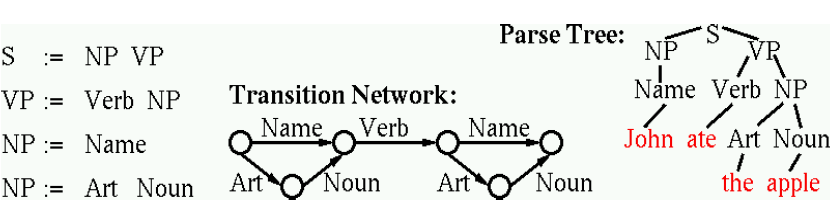
\includegraphics[width=10cm]{images/cfglm.png}
\caption{\label{fig:contextFreeGrammarLM} Context-free grammar language models.}
\end{figure}

\subsubsection{Tree-based language models}
$n$-grams have a very limited context and training the parameters is almost impossible for large values of $n$. We can use a CART-based technique (classification and regression trees), where every tree node asks about $k$ previous words ($k \approx 20$). Every leaf node is a unigram probability distribution on our vocabulary. This is somewhat similar to clustering acoustic context-dependent models ($\to$ figure~\ref{fig:treeBasedLM}).

\begin{figure}[htb]
\centering
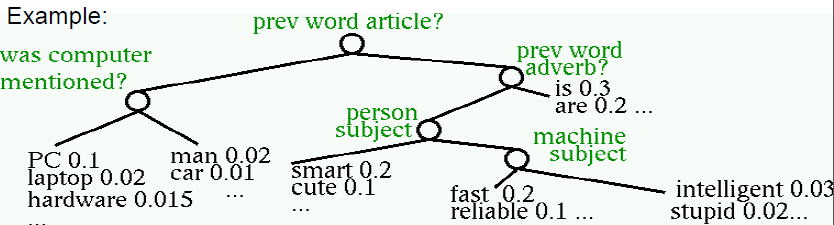
\includegraphics[width=10cm]{images/tblm.png}
\caption{\label{fig:treeBasedLM} Tree-based language models.}
\end{figure}

\subsubsection{HMMs for language modeling}

Often, speech is carried out in phases, such as \textit{greeting} $\rightarrow$ \textit{smalltalk} $\rightarrow$ \textit{good-bye}. Based on this, we can build an HMM, where every state emits language models or mixture weight distributions ($\to$ figure~\ref{fig:hmmLM}).

\begin{figure}[htb]
\centering
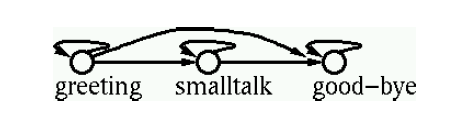
\includegraphics[width=10cm]{images/hmmlm.png}
\caption{\label{fig:hmmLM} HMMs for language modeling.}
\end{figure}

\subsection{Vocabulary selection}
A smaller vocabulary eliminates potentially confusing candidates and improves the word error rate. A larger vocabulary has a lower out-of-vocabulary rate, but the word error rate increases. The goal is to balance the WER and OOV rates. We do this by using a corpus of text to determine appropriate vocabularies. For example, we can pick data from a specific domain and use the most frequent words.

\subsection{$n$-gram pruning}
The size of higher-order $n$-gram models if often too large for practical applications. Therefore we reduce the size of $N$-gram models by \textbf{Pruning}. We minimize the relative entropy between original and pruned model and the performance loss.
Experience shows that trigram models can be pruned by more than 25\% without losing recognition accuracy.

\subsection{Problems with spontaneous speech}
\begin{itemize}
    \item silence between words (\textit{``hello world''} vs. \textit{``hello \hspace{5pt} world''})
    \item hesitations (\textit{``ah''}, \textit{``uhm''}, ...)
    \item filler words an phrases (\textit{``I mean''}, \textit{``you know''}, ...)
    \item false starts, aborts, etc. (\textit{``let's meet sun- no saturday''})
    \item non-verbal sounds (breathing, lip smacks, ...)
\end{itemize}

Possible solutions are:
\begin{itemize}
    \item just ignore it (\textit{duh!})
    \item increase context width (e.g. use $4$-grams instead of trigrams)
    \item skip spontaneous effects in the history
\end{itemize}

\subsection{Unknown words}

\vspace{5pt}
\textit{\textbf{Note:} Here, ``unknown word'' refers to a word not seen in the training data, but occuring in the decoder vocabulary and dictionary - as opposed to not being known at all.}
\vspace{10pt}

In the acoustic model, we can handle words that have not been seen in the training set by defining their pronunciation(s) in the pronunciation lexicon. However, in most speech recognition tasks, we cannot train all words that might have to be recognized some time. So, how do we incorporate unknown words into the language model? 
Approaches to this problem include:
\begin{itemize}
    \item rewrite all words in the training text that only occur one with UNK and treat every unknown word in the recognition run as UNK
    \item use a class-based language model and assign a class to every unknown word
    \item add new word into vocabulary and use cache language model to improve the parameters for subsequent recognitions
\end{itemize}

\subsection{OOV words}
OOV words are words that are not known at all. These words \textit{must} lead to recognition errors. Ideally, every OOV word causes only one substitution, which would imply WER = OOV. Usually, there are follow-up errors: every OOV word causes between 1.5 and 2 errors on average.

\subsection{Problems with different languages}
\begin{itemize}
    \item \textbf{Problem:} Highly inflecting languages pose more of a problem to language recognition. \textbf{Solution:} Use morpheme-based language models.
    \item \textbf{Problem:} Some languages, e.g. German allow arbitrary compounding of nouns. \textbf{Solution:} Decompose compound nouns.
    \item \textbf{Problem:} Some languages, e.g. Chinese have a different or no specified notion of words. \textbf{Solution:} Consider syllable-based language models.
\end{itemize}

\subsection{Problems with Recognition Errors}
Strong language model constraints can lead to follow-up errors: If a word is misrecognized, strong constraints can lead to the next word(s) to be misrecognized, too.
An approach to solve this issue may be to change the effect of the language model on the recognition process depending on the current confidence.


\subsection{Language model adaptation}
Natural language is highly variable, depending on time (medieval German vs. current German), domain (fishing vs. politics), context (scientific paper vs. chatting with friends), etc.

\begin{figure}[htb]
\centering
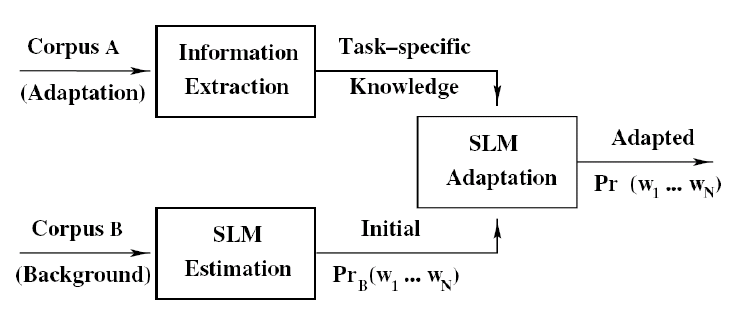
\includegraphics[width=10cm]{images/lmaf.png}
\caption{\label{fig:lmAdaptationFramework} Language model adaptation framework.}
\end{figure}

Generally, we have a large background corpus $\mathcal{B}$ and a small adaption corpus $\mathcal{A}$ depending on the current task. The goal is to compute a robust estimate of the language model probability $Pr(w_1,\dots,w_N) = \prod_{q=1}^{N} Pr(w_q | h_q)$, where $h_q = w_{q-n+1}, \dots, w_{q-1}$. We can try to solve this problem by using language model adaptation (see also figure~\ref{fig:lmAdaptationFramework}). There are three techniques of doing this:
\begin{itemize}
    \item Model Interpolation
    \item Constraint Specification
    \item Meta-Information Extraction
\end{itemize}

\subsubsection{Retrieval of adaptation data}
We have to retrieve our adaption data froms somehwere:
\begin{itemize}
    \item \textbf{Grammar-based system}: Generate text using the grammar. (Random rules or use small corpus to learn rule weights)
    \item \textbf{Use recognition output}: Accumulate corpus $\mathcal{A}$ during the recognition process, Take N-best or Confusion Networks as adaptation material;
each hypothesis contributes to corpus according to its posterior likelihood
    \item \textbf{Search \& Retrieve}: Use a small corpus $\mathcal{A}$ as a seed for retrieval techniques (online databases and WWW).
\item Augment data at the $N$-gram count level
\end{itemize}

\subsubsection{Model interpolation}
\textbf{Idea:} Derive task-specific (\emph{dynamic}) SLM from Corpus $\mathcal{A}$ and combine this with the background (\emph{static}) SLM from $\mathcal{B}$.
\begin{enumerate}
    \item \textbf{Linear Interpolation}: $P(w_q \bigm| h_q) = (1 - \lambda) \cdot P_A(w_q \bigm| h_q) + \lambda \cdot P_B(w_q \bigm| h_q)$
    \item \textbf{Backoff}:
        \[
            P(w_q \bigm| h_q) = \begin{cases}
                P_A(w_q \bigm| h_q) & \mbox{if } C(h_q w_q) \geq T \\
                \beta \cdot P_B(w_q \bigm| h_q) & \mbox{otherwise}
            \end{cases}
        \]
    \item \textbf{Dynamic Cache Model}: $P(w_q \bigm| h_q) = \sum\limits_{\left\{c_q\right\}} P(w_q \bigm| c_q) \cdot P(c_q \bigm| h_q)$
    \item \textbf{Maximum a-Posteriori}:
        \[
            P(w_q \bigm| h_q) = \frac{\epsilon \cdot C_A(h_qw_q) + C_B(h_qw_q)}{\epsilon \cdot C_A(h_q) + C_B(h_q)}
        \]
\end{enumerate}

\subsubsection{Constraint specification}
\textbf{Idea:} Extract features from corpus $\mathcal{A}$ that are used as constraints for the adapted SLM.
Constraint specification is more powerful than Model Interpolation since different weights could be assigned to each extracted feature separately.
\begin{enumerate}
\item \textbf{Exponential Models}: Historically constraint-based methods are associated with exponential models trained on Maximum Entropy (ME) criterion which leads to Minimum Discrimination Information estimation.
\item \textbf{MDI Adaptation}
\item \textbf{Unigram Constraints}
\end{enumerate}


\subsubsection{Meta-information extraction}
\textbf{Idea:} Use corpus $\mathcal{A}$ to extract background information about the underlying subject matter. Improve upon the background model based on semantic classification.
\begin{itemize}
\item Mixture Models
\item Semantic Knowledge
\item Syntactic Infrastructure
\begin{itemize}
\item Structured Language Models
\item Syntactic Triggers
\end{itemize}
\item Multiple Sources
\begin{itemize}
\item Combination Models
\item Whole sentence Models
\end{itemize}
\end{itemize}

\newpage

\section{Search}

\textbf{Isolated word recognition:}
\begin{itemize}
    \item for every applicable vocabulary word, compute it's score (DTW) and it's likelihood (Forward algorithm)
    \item report the word with the best score / likelihood
\end{itemize}

\vspace{5pt}

\textbf{Continuous speech recognition:}
\begin{itemize}
    \item not only find state sequence in words
    \item but also find the word sequence
\end{itemize}

\vspace{5pt}

\subsection{DTW optimization}
\begin{itemize}
    \item define start and end point
    \item path should be close to diagonal
    \item no two successive horizontal / vertical steps
    \item pruning: eliminate losers (with score $s < s_{best} - \Delta$)
    \item usually, we're only interested in the final score, so we can overwrite older values
\end{itemize}

Drawbacks of DTW include speaker dependency and inefficiency for large vocabularies.

\subsection{Viterbi optimization}
Use tree search ($\to$ figure~\ref{fig:viterbiTreeSearchOptimization}).
\begin{figure}[htb]
    \begin{minipage}{\linewidth}
        \vspace{5cm}
        \hfill \scriptsize search1.17
    \end{minipage}
    \caption{\label{fig:viterbiTreeSearchOptimization} Viterbi tree search optimization.}
\end{figure}

\subsection{Advanced optimization techniques}

\subsubsection{Two-level DTW}
\begin{enumerate}
    \item for each remotely likely word begin time, compute DTW with open end within all words
    \item for each word start and end times calculated in the previous step, combine words with DTW based on calculated scores
\end{enumerate}

Obviously, this is extremely costly for large vocabularies and longer words.

\subsubsection{Depth-first search}

Depth-first vs. breadth-first corresponds roughly to \textit{time-asynchronous} vs. \textit{time-synchronous}.

\textbf{$A^{\ast}$ search} (usually implemented with a stack decoder):

\subsubsection{Viterbi beam search vs. $A^{\ast}$ stack decoder}
Beam search doesn't require a heuristic and it is appropriate for parallel implementation. However, it is not admissible, that is it might not find the best solution. Nowadays, beam search is usually preferred over $A^{\ast}$ (though $A^{\ast}$ is taken for search through $n$-best and lattice structures).

\subsubsection{One stage dynamic programming}
Use Viterbi within words. For the first state of each word, consider the best last state of all words as predecessor. In order to reconstruct the best word sequence, find the best predecessor word to the current word. Finally backtrace.

\textit{\textbf{Note:} ???}

All search techniques use two strategies for efficiency:
\begin{itemize}
    \item \textbf{Sharing:} Keep intermediate results so that they can be reused by other paths without recomputation. For example, when computing the emission probabilities of \textit{``can''} and \textit{``cash''}, we can reuse the emission probabilities for the phonemes \textit{C} and \textit{AE}.
    \item \textbf{Pruning:} Disregard unpromising paths without wasting time exploring them further.
\end{itemize}

When using bigrams, the best predecessor depends only on the current word, this is possible by storing one backpointer for each active word end. When using trigrams, the best predecessor also depends on the successor of the current word. Then, things ``get ugly'' and we have to approximate a solution.

The transition into an initial state of a word $Z$ is computed by maximizing (Viterbi / DTW) the scores / accumulated distances $C(W)$ of all word-final states in the previous time frame and adding the local acoustic score $am(Z)$: e.g. $C(X) + am(Z)$ vs. $C(Y) + am(Z)$. When using a grammar, we additionally have to add to the accumulated score a language model score $lm(Z)$, e.g. $C(X) + am(Z) + lm(X, Z)$ vs. $C(Y) + am(Z) + lm(Y,Z)$. Without a grammar, the best predecessor state is the same for all word-initial states, whereas with a grammar, the best predecessor state also depends on the word transition probability.

\vspace{10pt}

When using tree search with a language model, we have a problem. After making a word-to-word transition, we don't know which word we are entering, but this knowledge is required to properly compute the probability of the transition. The solution to this are \textbf{delayed bigrams}. We make every word's final state unique. That way, we know which word we processed when we are in the final state. At that point, we can incorporate the language model information into our calculation (hence,
\textit{delayed}) ($\to$ figure~\ref{fig:delayedBigrams}).
\begin{figure}[htb]
    \begin{minipage}{\linewidth}
        \vspace{4cm}
        \hfill \scriptsize search2.15
    \end{minipage}
    \caption{\label{fig:delayedBigrams} Delayed bigrams.}
\end{figure}

\vspace{10pt}

\subsubsection{Unigram lookahead}
No bigram information can be included until word identity is known. Instead, we estimate the unigram information of the remainder subtree and include the bigram information as soon as possible (see also figure~\ref{fig:unigramLookahead}).
\begin{figure}[htb]
    \begin{minipage}{\linewidth}
        \vspace{4cm}
        \hfill \scriptsize search2.16
    \end{minipage}
    \caption{\label{fig:unigramLookahead} Unigram lookahead.}
\end{figure}

\vspace{10pt}

\subsubsection{Multi-pass searches}
Why use multiple passes in continuous speech recognition:
\begin{itemize}
    \item we could use a good estimator for $A^{\ast}$ search
    \item in pruning we could use a good lookahead to prune away the ``right'' parts
    \item recover from errors resulting from delayed bigrams
\end{itemize}
Forward-backward search: first, run backward pass, then run forward pass using backward scores to do pruning. Problems:
\begin{itemize}
    \item when using a search pass to compute information for pruning, it has to be a lot faster than the actual search pass
    \item it cannot produce better results than the actual search pass
    \item no runon recognition possible (start processing before sentence has finished)
    \item where do we get backward bigrams from?
\end{itemize}
Example for a multi-pass search: in the first pass, use a narrow beam and a fast but weak acoustic model to prune some paths. In the second pass, use a regular Viterbi search with a wider beam and a slower but more powerful acoustic model, considering that some areas have already been pruned in the first run.

\subsubsection{Multiple hypothesises}
Reasons:
\begin{itemize}
    \item do postprocessing on all hypothesises using additional knowledge
    \item speech understanding
    \item manual recovery options for the users
\end{itemize}
When recognizing isolated words, simply report not only the best, but the $n$ best results. In continuous speech recognition, we can either use multiple recognizers and report all their results, or let Viterbi not only remember the best predecessor, but the $n$ best predecessors.

A problem with multiple hypothesises is that the results are often quite similar in respect to their content words, while the non-content words are more variable. This results in many ``useless'' hypothesis. But if we simply increase $n$, the system may become too slow. The solution to this is to use \textbf{word lattices} ($\to$ figure~\ref{fig:wordLattice}).
\begin{figure}[htb]
    \begin{minipage}{\linewidth}
        \vspace{3cm}
        \hfill \scriptsize search2.22
    \end{minipage}
    \caption{\label{fig:wordLattice} A word lattice.}
\end{figure}

\newpage

\section{Text-to-speech synthesis}

Typically, text-to-speech synthesis involves three steps:
\begin{enumerate}
    \item \textbf{text analysis:} from strings of characters to words
    \item \textbf{linguistic analysis:} from words to pronunciations and prosody
    \item \textbf{waveform synthesis:} from pronunciations to waveforms
\end{enumerate}

We use the \textit{mean mel cepstral distortion} (\textbf{MCD}) as a quality measure (smaller is better).

\subsection{Text analysis}
\begin{itemize}
    \item character encodings
    \item word segmentation
    \item numbers, symbols, non-standard words
        \begin{itemize}
            \item anything not directly in the lexicon
            \item OOV or novel forms
            \item abbreviations, letter sequences, acronyms
        \end{itemize}
    \item may require special rules
        \begin{itemize}
            \item train rules for homographs
            \item numbers, roman numerals
        \end{itemize}
\end{itemize}
Text processing errors are the most common complaints in TTS. Examples:
\begin{itemize}
    \item ``My cat who \textit{lives} dangerously has nine \textit{lives}.''
    \item ``He stole \textit{\$}100 from the bank.''
    \item ``He stole \textit{1996} cattle on 25 Nov. \textit{1996}.''
    \item ``It's 13 \textit{St.} Andrew \textit{St.} near the bank.''
\end{itemize}
We employ a ``bunch of hacky rules'':
\begin{itemize}
    \item \textbf{splitter:} domain-independent tokenizer
    \item \textbf{token type classifier:} identify numbers and abbreviations, disambiguate homographs
    \item \textbf{token type expander}
    \item \textbf{language model}
\end{itemize}

\subsection{Linguistic analysis}

The lexicon should be as comprehensive as possible, but this is impossible. So, we have to pronounce OOV words, too.

\subsubsection{Bootstrapping}

\begin{enumerate}
    \item select some frequently occuring words and build lexical entries from them
    \item select an article of text
    \item synthesize each unknown word, add correct words to list
    \item repeat
\end{enumerate}

\subsection{Waveform synthesis}
Concatinative synthesis:
\begin{itemize}
    \item random word / phrase concat
    \item phone concat
    \item diphone concat ($\left|\mbox{phones}\right|^2$ transitions)
    \item sub-word unit selection
    \item cluster-based unit selection
\end{itemize}

\newpage

\section{Spoken dialog systems}

A dialog is a verbal interaction of two or more agents over more than one utterance in order to establish a joint goal. A spoken dialog system is an autonomous, artificial system that engages in a dialog with a human and employs speech recognition and synthesis. Commonly, a complete interaction is referred to as a \textit{session}, an \textit{utterance} is one person's speech between two pauses, and a \textit{turn} represents all utterances of one partner, until the other partner starts interacting. A \textit{barge-in} happens when a turn is interrupted.
There are two kinds of initiatives, the \textit{system initiative}, e.g. ``Please tell me your destination airport.'' (more rigid, less ASR errors) or the \textit{mixed initiative}, e.g. ``What flight are you interested in?'' (less rigid, harder to recognize and understand).

\begin{figure}[htb]
    \begin{minipage}{\linewidth}
        \vspace{5cm}
        \hfill \scriptsize sds.7
    \end{minipage}
    \caption{\label{figureA} Components of a spoken dialog system.}
\end{figure}

A \textit{discourse} is the entirety of information and structure of the ongoing dialog up to a certain point. Each new utterance must be interpreted in the light of the ongoing discourse and then included in it.

\vspace{5pt}

In order to represent a discourse, Montague grammars are commonly used (transform text into first order logic). Problem: ``A man walks in the park. He whistles'' $\rightarrow (\exists x : man(x) \wedge walksinpark(x)) \wedge (\exists x : whistles(x))$. What we need is \textit{anaphora resolution}.

\vspace{5pt}

Don't forget \textit{typed feature structures}. We can build \textit{semantic grammars} with it.

\vspace{5pt}

\textbf{Dialog strategies:}
\begin{itemize}
    \item \textbf{plan-based} system: the idea is that communication is the result of a plan (to do / achieve something)
    \item \textbf{grammar-based} system: there are adjacency pairs, such as \textit{question} $\rightarrow$ \textit{answer}, \textit{proposal} $\rightarrow$ \textit{acceptance}, etc.
    \item \textbf{finite-state grammars:} describe possible events with a finite state automata (simple to produce, but rigid)
    \item \textbf{rational agency:} formally describe rational behavior and then use formal proofs in order to deduce next steps
    \item \textbf{frame-based} systems: somewhat similar to web forms, additionally define \textit{moves} (which may contain \textit{conditions}) to ask for specific information
    \item \textbf{statistical systems:} learn optimal next system action from corpus of completed dialogs
\end{itemize}

\vspace{5pt}

The dialog system has to communicate with the ASR system. Returning only the best hypothesis is usually not sufficient. We may have to weigh hypothesises according to the dialog act expectations. Also, we should adapt the context to each turn (e.g. in a navigation system in Karlsruhe, \textit{``Durlach``} will be more likely than \textit{``Paris''}, which is different from most other contexts).

\vspace{5pt}

If our system is \textit{multimodal}, we can also use gestures, etc.

\newpage

\section{Multilingual speech processing}

We can't simply retrain on foreign data, because:
\begin{itemize}
    \item different scripts, no vowelization, no writing system
    \item no word segmentation, rich morphology
    \item tonality, click sounds
    \item social factors such as trust, access, exposure and cultural background
\end{itemize}
For an overview of the system, see figure~\ref{fig:overviewMSPS}.

\begin{figure}[htb]
    \begin{minipage}{\linewidth}
        \vspace{7cm}
        \hfill \scriptsize msp2.4
    \end{minipage}
    \caption{\label{fig:overviewMSPS} Overview of multilingual speech processing systems.}
\end{figure}

Let's try to build a language independent ASR system!
\begin{itemize}
    \item language independent acoustic modeling
        \begin{itemize}
            \item \textit{International Phonetic Alphabet} easy to implement, easy to port to other languages
            \item fully data-driven procedure
        \end{itemize}
    \item universal language model: combine LMs of different languages to allow code switching
\end{itemize}

\vspace{10pt}
\textbf{Multilingual acoustic modeling}
\vspace{10pt}

\begin{enumerate}
    \item \begin{itemize}
            \item uniform multilingual speech database
            \item monolingual recognizers for many languages
        \end{itemize}
    \item \begin{itemize}
            \item combine monolingual acoustic models
            \item share data across languages
        \end{itemize}
\end{enumerate}

\vspace{10pt}
\textbf{Acoustic model combination}
\vspace{10pt}

Sound production is \textit{human}-specific, not \textit{language}-specific. Thus, it is sufficient to represent sounds with the IPA.
\begin{enumerate}
    \item build universal sound inventory based on IPA (485 sounds $\rightarrow$ 162 IPA sound-classes)
    \item each sound class is represented by one phoneme which is trained through data sharing:
        \begin{itemize}
            \item \textit{m}, \textit{n}, \textit{s}, \textit{l} occur in all languages
            \item \textit{a}, \textit{e}, \textit{i}, \textit{o}, \textit{u} and \textit{p}, \textit{b}, \textit{t}, \textit{d}, \textit{k}, \textit{g}, \textit{f} occur in most languages
            \item some data is not shared
        \end{itemize}
\end{enumerate}

\vspace{10pt}
\textbf{Challenges}
\vspace{5pt}

\begin{itemize}
    \item Many ASR algorithms are language independent, but they require lots of training data. For many languages, not a lot of training data exists, so we need a different approach. For example, we might use intelligent learning systems.
    \item The contexts of sounds are language specific. How can we still use context dependent modeling?
        \begin{itemize}
            \item multilingual decision context trees
            \item specialize decision tree by adaptation
        \end{itemize}
\end{itemize}

\vspace{10pt}
\textbf{Web-derived pronunciations}
\vspace{5pt}

\vspace{10pt}
\textbf{Unsupervised training}
\vspace{5pt}

Idea: decode untranscribed audio data, select data with high confidence, use selected data to train / adapt recognizer.

\newpage
\section{Prüfungsfragen}
\subsection{Allgemeine Fragen}
\begin{itemize}
\item Was ist MMMK? Wofür steht MMMK?
\begin{itemize}
\item \emph{Multilinguale Mensch-Maschine Kommunikation}
\end{itemize}
\item Wo findet MMMK Anwendung?
\begin{itemize}
\item \emph{Interaktion mit einem Computer/Maschine  mittels natürlicher Sprache}
\end{itemize}
\item Vor- und Nachteile gegenüber anderen Kommunikationsmitteln
\begin{itemize}
\item \emph{siehe Vor- und Nachteile im Kapitel 1} %variabel machen
\end{itemize}
\item Welche Probleme können dabei auftreten?
\item Zeichnen sie das Blockschaubild (Young oder Schultz)
\begin{itemize}
\item \emph{siehe Overview Figure 1 und 2} % variabel referenzieren 
\end{itemize}
\item Geben Sie die Fundamentalformel (nach Bayes) an.
\begin{itemize}
\item $\hat{W} = argmax_{W} P(W | X) = argmax_{W} \frac{P(X|W) \cdot P(W)}{P(X)}$ 
\end{itemize}
\item Beschreiben Sie den Zusammenhang zwischen Fundamentalformel und Blockschaltbild.
\begin{itemize}
\item\emph{$P(X|W)$ kommt vom Akustischen Modell, $P(W)$ vom Sprachmodell, $P(X)$ ist die a-priori Wahrscheinlichkeit, 
$argmax$ ist der Decoder und $\hat{W}$ die wahrscheinlichste Hypothese.}
\end{itemize}
\item Was ist an Umgangssprache so schlimm?
\begin{itemize}
\item \emph{Grammatisch oft inkorrekt, Aussprache ggf. undeutlich bzw. untypisch}
\end{itemize}
\item Was ist Co-Artikulation?
\begin{itemize}
\item Wenn die Aussprache eines Phonems/Wortes durch den umgebenden Kontext verändert wird.
\end{itemize}
\item Was ist ein Phonem? 
\begin{itemize}
\item Kleinste Bedeutungsunterscheidende akkustische Einheit
\end{itemize}
\item Wie werden false starts modelliert? 
\begin{itemize}
\item Als Hypothese bekommt man genau das raus, was gesagt wurde inklusive aller Mhms und Ähs.
\end{itemize}
\end{itemize}

\subsection{Vorverarbeitung}
\begin{itemize}
\item Erklären sie die Funktionsweise eines Kondensatormikrophons.
\begin{itemize}
\item \emph{Zwei Membranen, eine dicke und eine dünne, die als Plattenkondensator fungieren. Die dünne Membran wird durch Schalldruckwellen angeregt und schwingt. Durch die Kapazitätsänderung kommt es zu einer messbaren Spannungsänderung.}
\end{itemize}
\item Was macht man bei der Vorverarbeitung?
\begin{itemize}
\item Tiefpassfilter (Anti-Alias-Filter)
\item Abtasten (Sampling) [X-Achse diskret machen]
\item Quantisieren [Y-Achse diskret machen]
\item Fenstern
\item Fouriertransformation um an Frequenzinformation zu gelangen
\item Filterbänke anwenden zur Reduzierung der Dimension
\item Logarithmieren (um einfacherer den Kanal loszuwerden)
\item inverse Fouriertransformierte berechnen
\item Ergebnis: Cepstralkoeffizienten
\item Alternative: Linear Predictive Coding (berechne aus bisherigen Signalwerten die dann kommenden)
\end{itemize}
\item Was ist ein Vorteil vom Cepstrum? 
\begin{itemize}
\item Der Vokaltrakt ist bei allen Menschen etwa gleich und daher sind die Cepstralkoeffizienten relativ robust und sprecherunabhängig.
\end{itemize}
\item Was muss beim Abtasten (Sampling) beachten?
\begin{itemize}
\item \emph{Shannon-Nyqist-Theorem: Abtastfrequenz muss echt größer als der doppelten Signalfrequenz sein.}
\end{itemize}
\item Was machen Quantisierung und Sampling?
\begin{itemize}
\item \emph{Quantisierung diskretisiert die Y-Achse und Sampling die X-Achse.}
\end{itemize}
\item Was für ein Filter wird beim Sampling benötigt und warum?
\begin{itemize}
\item \emph{Tiefpassfilter, da wir ein bandbegrenztes Signal brauchen.}
\end{itemize}
\item In welchem Frequenzbereich hört der Mensch?
\begin{itemize}
\item \emph{bis zu 32k Hz, Abtastfrequenz ist üblicherweise 8kHz}
\end{itemize}
\item Warum wollen wir die Frequenzinformation haben?
\begin{itemize}
\item \emph{Das Ohr macht das auch so.}
\end{itemize}
\item Was macht man nach dem Digitalisieren des Signals?
\begin{itemize}
\item \emph{Nach der Digitalisierung wird das Signal gefenstert.}
\end{itemize}
\item Was für Fensterformen gibt es?
\begin{itemize}
\item Rectangle, Gaussian, \textbf{Hamming}, Hanning
\end{itemize}
\item Was wird beim Fenstern gemacht? Und warum wird das Signal gefenstert?
\begin{itemize}
\item Man multipliziert das Signal mit einem Finite-Duration-Window und berechnet dann die DTFT. Das muss gemacht werden, da man ansonsten die zeitlichen Informationen nach der FT verlieren würde.
\end{itemize}
\item Wieso muss man anschließend das Signal noch filtern? Was ist die Mel-Filterbank? 
\begin{itemize}
\item Viele der Fourierkoeffizienten enthalten redundante oder gar irreführende Informationen über die Mikrostruktur. Diese werden nicht benötigt. So reduziert man die Dimensionalität. \dots
\end{itemize}
\item Wie trennt man das stimulierende Signal von der "impulse response"?
\begin{itemize}
\item Es gilt $s(n) = u(n) *  h(n)$. \\ $\rightarrow_{FT} F(s) = F(u) \cdot F(h)$ \\ $\rightarrow_{LOG} F^{-1}(log(F(s))) = F^{-1}(log(F(u))) + F^{-1}(log(F(h)))$
\end{itemize}
\item Was ist MFCC? Und LPC?
\begin{itemize}
\item MFCC (Mel-Filter-Cepstral-Coefficients) bzw. Linear Predictive Coding, s. Skript
\end{itemize}
\item Was macht man mit einem Featurevektor? 
\begin{itemize}
\item Berechnen der Deltas und DeltaDeltas um Zeitinformationen zu erlangen.
\end{itemize}
\item Erläutere das Quelle-Filter-Model (Source-Filter Model). 
\begin{itemize}
\item s. Skript
\end{itemize}
\end{itemize}


\subsection{Akkustisches Modell}
\begin{itemize}
\item Zeichne HMM für ein Phonem/Wort.
\begin{itemize}
\item \emph{siehe HMMs}
\end{itemize}
\item Was für Topologien gibt es? Welche wird üblicherweise verwendet?
\begin{itemize}
\item \emph{Linear, Left-to-Right, Alternative paths, Ergodic, \textbf{Bakis}}
\end{itemize}
\item Warum benötigen HMMs 3 Zustände pro Phonem?
\begin{itemize}
\item \emph{Beginn, Mitte, Ende}
\end{itemize}
\item Woraus setzt sich eine HMM zusammen?
\begin{itemize}
\item Fünftupel $(S, \pi, A, B, V)$:
\begin{itemize}
\item Zustandsmenge $S = \{s_1,s_2,\dots,s_n\} - n$ is the number of states
\item Initiale Wahrscheinlichkeitsverteilung $\pi(s_i) = P(q_1 = s_i)$
\item Matrix der Zustandsübergangswahrscheinlichkeiten $1 \le i, j \le n, $\\ $A = (a_{ij}), a_{ij} = P(q_{t+1} = s_j | q_t = s_i)$
\item Menge der Emissionswahrscheinlichkeiten $B = \{b_1, \dots, b_n\}, b_i(x) = P(o_t = x | q_t = s)$
\item Symbolmenge $V = \{x_1,x_2,\dots,x_v\}$ (discrete) or $V = R^d$ (continuous)
\end{itemize}
\end{itemize}
\item Was sind die drei Hauptprobleme von HMMs und mit welchem Algorithmus kann man sie jeweils lösen?
\begin{itemize}
\item \emph{Evaluation (Forward), Decoding (Viterbi) und Learning Problem (Forward-Backward Algortihm / Baum-Welsch) [ausführliche Erklärung der Probleme und Algorithmen s. Skript]}
\end{itemize}
\item Schreiben Sie [Forward/Viterbi/Forward-Backward/Baum-Welch] mit sämtlichen Formeln auf und erklären Sie die Vorgehensweise und Unterschiede.
\begin{itemize}
\item \emph{s. Skript}
\end{itemize}
\item Was steht in einem Pronounciation Dictionary?
\begin{itemize}
\item eine Liste von Wörtern mit zugehörigen Aussprachmöglichkeiten
\end{itemize}
\item Wie sind die HMMs gestaltet, sodass man mit weniger Trainingsdaten bessere Ergebnisse erzielt?
\begin{itemize}
\item \emph{Die bei den Emissionswahrscheinlichkeiten verwendeten Gaußverteilungen werden kombiniert und verschieden gewichtet.}
\end{itemize}
\item Wie verbindet man mehrere Wörter hintereinander?
\begin{itemize}
\item (Sprachmodell)
\end{itemize}
\item Wie lange ist man mindestens in einem State? 
\begin{itemize}
\item 10ms
\end{itemize}
\item Woher bekommt man die HMMs? 
\begin{itemize}
\item Im Pronounciation Dictionary steht, aus welchen Phonemen ein Wort besteht. Das baut man dann für die Wörter zusammen.
\end{itemize}
\item Nenne ein Beispiel in dem Viterbi und Forward-Algorithmus nicht zum gleichen Ergebnis kommen. 
\begin{itemize}
\item viele Pfade mit ähnlicher Wahrscheinlichkeit, der wahrscheinlichste führt zu Wort X, alle anderen zu Y. Viterbi findet X, Forward findet Y
\end{itemize}
\item Wie trainiert man HMMs? 
\begin{itemize}
\item Mit einem Expectation-Maximation-Algorithmus (EM-Algorithmus), wie beispielsweise Baum-Welch.
\end{itemize}
\item Durch welche Parameter sind Gaußmixturverteilungen definiert? 
\begin{itemize}
\item Mittelwert, Varianz und Mixturgewicht
\end{itemize}
\item Welche Probleme können bei HMMs in der Modellierung im Sprachmodell auftreten? 
\begin{itemize}
\item Beim Eintritt in die HMM weiß man noch nicht, in welchem Wort man ist. Das ist bspw. für Bigramme schlecht. Daher verwendet man Delayed-Bigrams.
\end{itemize}
\item Wie kann man Koartikulation modellieren? 
\begin{itemize}
\item Jedes Phonem für jeden Kontext modellieren. Zu viele Kontexte, also Kontexte in Klassen zusammenfassen, via bottom-up oder top-down.
\end{itemize}
\item Wie kann man Viterbi (u.ä. Algorithmen) optimieren? 
\begin{itemize}
\item Beam Search
\end{itemize}
\item Wie können unterschiedliche Aussprachevarianten modelliert werden? (Bsp.: T in True und Tall)
\begin{itemize}
\item Markieren im Dictionary ODER Triphone (s. Skript)
\end{itemize}
\item Wie funktioniert Top-Down oder Bottom-Up Clustering 
\begin{itemize}
\item s. Skript
\end{itemize}
\end{itemize}


\subsection{Sprachmodell}
\begin{itemize}
\item Was ist der Unterschied zwischen einem deterministischen und einem stochastischen Sprachmodell?
\begin{itemize}
\item \emph{In einem deterministischen LM [Grammatik] hat ist $P(W)$ für jede Wortsequenz $W$ entweder 1 oder 0. In einem stochastischen ist $P(W)$ eine Wahrscheinlichkeit.}
\end{itemize}
\item Geben Sie die Wahrscheinlichkeit für ein N-Gram an.
\begin{itemize}
\item $P(w_k | w_1w_2\dots w_{k-1}) = P(w_k | w_{k-(n-1)}w_{k-(n-2)}\dots w_{k-1})$
\end{itemize}
\item Wie werden die anfangs berechnet? 
\begin{itemize}
\item Man nimmt einen großen Textcorpus und zählt die Häufigkeiten. $P(w|history) = \frac{Count(history \cdot w)}{Count(history)}$
\end{itemize}
\item Was ist Smoothing?
\begin{itemize}
\item \emph{Allen Zeicheketten wird eine Wahrscheinlichkeit ungleich 0 zugewiesen um ASR Fehler zu vermeiden.}
\end{itemize}
\item Welche Smoothing-Verfahren gibt es?
\begin{itemize}
\item \emph{Add-One, Backoff Smoothing (Absolute discounting, Katz, Kneser-Ney) und Linear Interpolation (Deleted interpolation) [ausführliche Erklärungen der Verfahren s. Skript]}
\end{itemize}
\item Wie funktioniert Class-Based Interpolation? 
\begin{itemize}
\item s. Skript
\end{itemize}
\end{itemize}

\newpage

\begin{figure}
\centering
\textbf{Danksagung} \\
\textbf{Guido Brückner} für die Kapitel Overview, Basics, Signal processing, Hidden Markov Models, Acoustic modeling, Language modeling, Search, Text-to-speech synthesis, Spoken dialog systems und Multilingual speech processing
\end{figure}

